% Created 2022-07-11 Mon 17:05
% Intended LaTeX compiler: pdflatex
\documentclass[presentation,aspectratio=169]{beamer}
\usepackage[utf8]{inputenc}
\usepackage[T1]{fontenc}
\usepackage{graphicx}
\usepackage{grffile}
\usepackage{longtable}
\usepackage{wrapfig}
\usepackage{rotating}
\usepackage[normalem]{ulem}
\usepackage{amsmath}
\usepackage{textcomp}
\usepackage{amssymb}
\usepackage{capt-of}
\usepackage{hyperref}
\usepackage{khpreamble}
\usepackage{amssymb}
\usepackage{tcolorbox}
\DeclareMathOperator{\shift}{q}
\DeclareMathOperator{\diff}{p}
\usetheme{default}
\author{Kjartan Halvorsen}
\date{2022-07-06}
\title{Relative stability}
\hypersetup{
 pdfauthor={Kjartan Halvorsen},
 pdftitle={Relative stability},
 pdfkeywords={},
 pdfsubject={},
 pdfcreator={Emacs 26.3 (Org mode 9.4.6)}, 
 pdflang={English}}
\begin{document}

\maketitle

\section{Root locus}
\label{sec:orgfe0ae11}
\begin{frame}[label={sec:org0dbae68}]{Root locus}
The rules for drawing the root locus is the same in continous as in discrete time. But the interpretation differs.
\begin{center}
\begin{tabular}{ll}
Continuous time & Discrete time\\
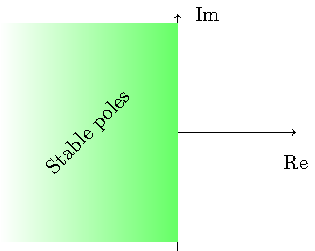
\includegraphics[width=0.28\linewidth]{../../figures/cont-stable} & 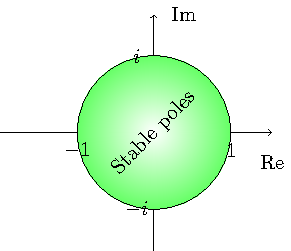
\includegraphics[width=0.28\linewidth]{../../figures/discrete-stable}\\
\end{tabular}
\end{center}
\end{frame}


\begin{frame}[label={sec:org361ed5e}]{Example: Position servo for the hard disk drive arm}
\begin{center}
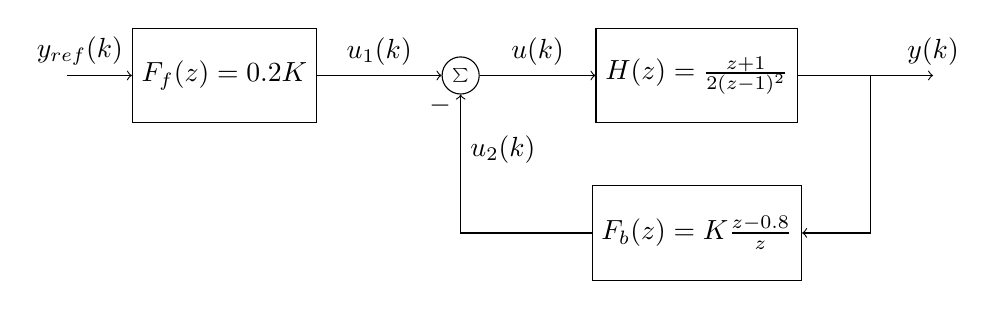
\begin{tikzpicture}
\tikzset{node distance=2cm, 
    block/.style={rectangle, draw, minimum height=12mm, minimum width=14mm},
    sumnode/.style={circle, draw, inner sep=2pt}        
}

  \node[coordinate] (input) {};
  \node[block, right of=input] (TR) {$F_f(z) = 0.2K$};
  \node[sumnode, right of=TR, node distance=30mm] (sum) {\tiny $\sum$};
  \node[block,right of=sum, node distance=30mm] (plant) {$H(z) = \frac{z+1}{2(z-1)^2}$};
  %\node[sumnode, right of=plant, node distance=30mm] (sumdist) {$\sum$};
  %\node[coordinate, above of=sumdist, node distance=15mm] (dist) {};
  %\node[coordinate, right of=sumdist, node distance=15mm] (measure) {};
  \node[coordinate, right of=plant, node distance=30mm] (output) {};
  \node[coordinate, right of=plant, node distance=22mm] (measure) {};
  %\node[sumnode,below of=measure, node distance=25mm] (sumnoise) {$\sum$};
  %\node[coordinate, right of=sumnoise, node distance=15mm] (noise) {};
  \node[block,below of=plant, node distance=20mm] (SR) {$F_b(z)=K\frac{z-0.8}{z}$};
  \draw[->] (input) -- node[above, pos=0.2] {$y_{ref}(k)$} (TR);
  \draw[->] (TR) -- node[above] {$u_1(k)$} (sum);
  \draw[->] (sum) -- node[above] {$u(k)$} (plant);
  \draw[->] (plant) -- node[at end, above] {$y(k)$} (output);
  \draw[->] (measure) |- (SR);
  \draw[->] (SR) -| (sum) node[right, pos=0.8] {$u_2(k)$} node[left, pos=0.96] {$-$};
\end{tikzpicture}
\end{center}

\alert{Characteristic equation}
\begin{align*}
1 + H(z)F_b(z) &= 0\\
1 + \frac{z+1}{2(z-1)^2}K\frac{z-0.8}{z} &= 0\\
(z-1)^2z + \frac{K}{2}(z+1)(z-0.8) &= 0
\end{align*}

\alert{For which values of \(K\) will the system be stable?}
\end{frame}

\begin{frame}[label={sec:org5d0918a}]{Example: Position servo for the hard disk drive arm}
\alert{Activity} Complete the root locus!
\[(z-1)^2z + \frac{K}{2}(z+1)(z-0.8) = 0\]
\begin{center}
  \begin{tikzpicture}[scale=2.5]
    \draw[->] (-1.2, 0) -- (1.2,0);
    \draw[->] (0, -1.2) -- (0,1.2);
    \node[red, pin=45:{2 process poles}] at (1,0) {\large $\times$};
    \node[red, pin=135:{Controller pole}] at (0,0) {\large $\times$};
    \node[green!70!black, pin=-145:{Controller zero}] at (0.8,0) {\Large $\circ$};
    \node[green!70!black, pin=-145:{Process zero}] at (-1,0) {\Large $\circ$};
    \node at (0.8, -0.2) {$0.8$};
    \node at (1, -0.2) {$1$};
    \draw[domain=0:360, samples=361, dashed] plot ({cos(\x)}, {sin(\x)});
    \node[coordinate, pin=60:{$|z|=1$}] at (0.5, 0.87) {};
  \end{tikzpicture}
\end{center}
\end{frame}


\section{Relative stability}
\label{sec:org5774b12}
\begin{frame}[label={sec:orgf53af3c}]{Relative stability}
\end{frame}

\begin{frame}[label={sec:orgea5be32}]{Sinusoid in - sinusoid out}
\begin{center}
  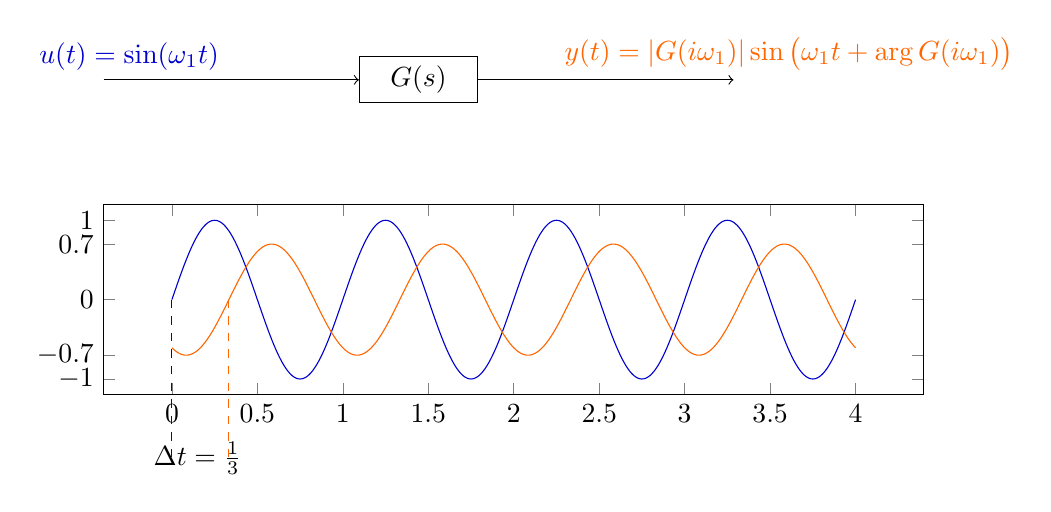
\begin{tikzpicture}[node distance=22mm, block/.style={rectangle, draw, minimum width=15mm}, sumnode/.style={circle, draw, inner sep=2pt}]

    \node[coordinate] (input) {};
    \node[block, right of=input, node distance=40mm] (plant)  {$G(s)$};
    \node[coordinate, right of=plant, node distance=40mm] (output) {};

    \draw[->] (input) -- node[above, pos=0.1, color=blue!80!black] {$u(t)=\sin(\omega_1 t)$} (plant);
    \draw[->] (plant) -- node[above, pos=0.3, anchor=south west, color=orange!80!red] {$y(t)=|G(i\omega_1)|\sin\big( \omega_1 t + \arg G(i\omega_1)\big)$} (output);


    \begin{axis}[
      yshift=-4cm,
      width=12cm,
      height=4cm,
      clip=false,
      ytick ={-1,-0.7, 0, 0.7, 1},
      ]
      \addplot[blue!80!black, no marks, domain=0:4, samples=600] {sin(360*x)};
      \addplot[orange!80!red, no marks, domain=0:4, samples=600] {0.7*sin(360*x - 120)};
      \draw[dashed, blue!80!black] (axis cs: 0, 0) -- (axis cs: 0, -2);
      \draw[dashed, orange!80!red] (axis cs: 0.333, 0) -- (axis cs: 0.333, -2);
      \node at (axis cs: 0.15, -2) {$\Delta t=\frac{1}{3}$};
    \end{axis}
  \end{tikzpicture}
  \end{center}
\(\omega_1 = \frac{2\pi}{T} = 2\pi\), \(|G(i\omega_1)| = 0.7\), \(\arg G(i\omega_1) = -\omega_1 \Delta t = -2\pi \frac{1}{3} = - \frac{2\pi}{3}\)
\end{frame}
\begin{frame}[label={sec:orga6430b4}]{If the phase shift is \(\pi\)}
\(G_o(i\omega_1) = -1\), \(|G_o(i\omega_1)| = 1\), \(\arg G_o(i\omega_1) = -\pi\)

\begin{center}
  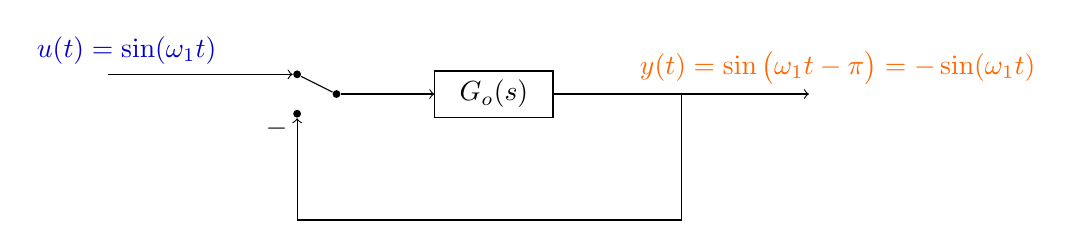
\begin{tikzpicture}[node distance=22mm, block/.style={rectangle, draw, minimum width=15mm}, sumnode/.style={circle, draw, inner sep=2pt}]

    \node[coordinate] (input) {};
    \node[circle, fill, inner sep=1pt, right of=input, node distance=24mm] (sum) {};
    \node[circle, fill, inner sep=1pt, below of=sum, node distance=5mm] (sum2) {};
    \node[coordinate, below of=sum, node distance=2.5mm] (summid) {};
    \node[circle, fill, inner sep=1pt, right of=summid, node distance=5mm] (sum3) {};
    \node[block, right of=sum3, node distance=20mm] (plant)  {$G_o(s)$};
    \node[coordinate, right of=plant, node distance=40mm] (output) {};

    \draw[->] (input) -- node[above, pos=0.1, color=blue!80!black] {$u(t)=\sin(\omega_1 t)$} (sum);
    \draw[->] (plant) -- node[coordinate, pos=0.5] (measure) {} node[above, pos=0.3, anchor=south west, color=orange!80!red] {$y(t)=\sin\big(\omega_1 t -\pi\big) = -\sin(\omega_1 t)$} (output);
    \draw[->] (sum3) -- node[above] {} (plant);
    \draw[->] (measure) -- ++(0,-16mm) -| node[pos=0.95, left] {$-$} (sum2);
    \draw (sum) to (sum3);
  \end{tikzpicture}
\end{center}

Closed-loop transfer function: \(G_c(s) = \frac{G_o(s)}{1 + G_o(s)}\)
\begin{tcolorbox}
We want \[ 1 + G_o(i\omega) \neq 0, \quad \forall \omega \]
If not, then the closed-loop system will have poles on the imaginary axis (in the s-domain). 
\end{tcolorbox}
\end{frame}

\begin{frame}[label={sec:org882c548}]{The simplified Nyquist criterion in the s-plane}
\begin{center}
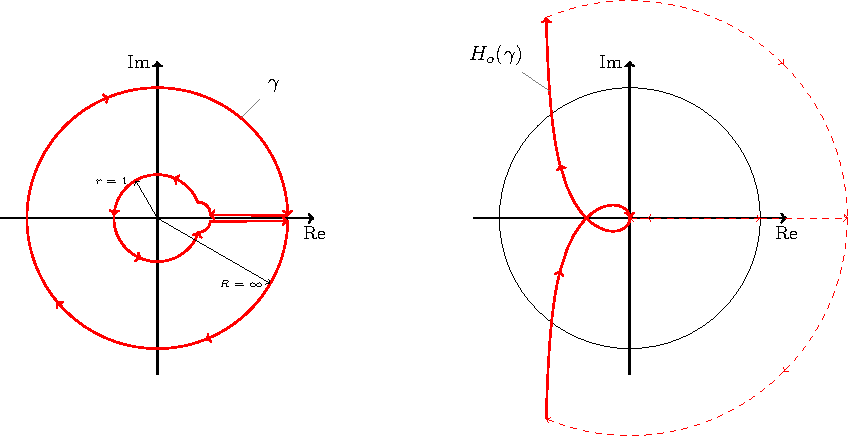
\includegraphics[width=0.65\linewidth]{../../figures/implane-nyquist-contour-map}
\end{center}

\pause

\begin{tcolorbox}
If the open-loop system (the loop gain) is not unstable, i.e. $G_o(s)$ has no poles in the right-half plane, then the closed-loop system will be stable if the Nyquist curve \textbf{do not encircle the point \(s=-1\)}. The point $s=-1$ should stay on the left side of the Nyquist curve when we go along the curve from low to high frequencies.
\end{tcolorbox}
\end{frame}

\begin{frame}[label={sec:orgc4aedc1}]{Stability margins}
\begin{center}
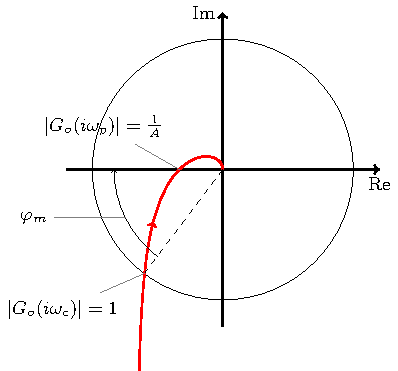
\includegraphics[width=0.38\linewidth]{../../figures/implane-nyquist-margins}
\end{center}
\begin{itemize}
\item Cross-over frequency: The frequency \(\omega_c\) for which \(|G_o(i\omega)| = 1\).
\item Phase margin: The angle \(\varphi_m\) to the negative real axis for the point where the Nyquist curve intersects the unit circle. \[\varphi_m = \arg G_o(i\omega_c) - (-180\degree) = \arg G_o(i\omega_c) + 180\degree\]
\end{itemize}
\end{frame}
\begin{frame}[label={sec:orgfc56374}]{Stability margins}
\begin{center}
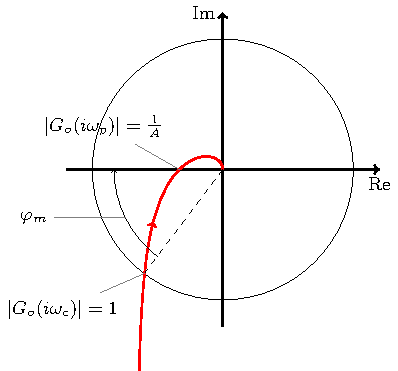
\includegraphics[width=0.38\linewidth]{../../figures/implane-nyquist-margins}
\end{center}
\begin{itemize}
\item phase-cross-over frequency: The frequency \(\omega_p\) for which \(\arg G_o(i\omega) = -180\degree\).
\item Gain margin: The gain \(K=A\) that would make the Nyquist curve of \(KG_o(i\omega h)\) go through the point \(-1 + i0\). This means that \[ |G_o(i\omega_p h| = \frac{1}{A}. \]
\end{itemize}
\end{frame}



\begin{frame}[label={sec:org9f31edf}]{The effect of sampling on the stability margins}
\[G(s) = \frac{1}{s^2 + 1.4s + 1} \quad \overset{h=0.4}{\longrightarrow} \quad H(z) = \frac{0.066z + 0.055}{z^2 - 1.450z + 0.571}\] 
\begin{center}
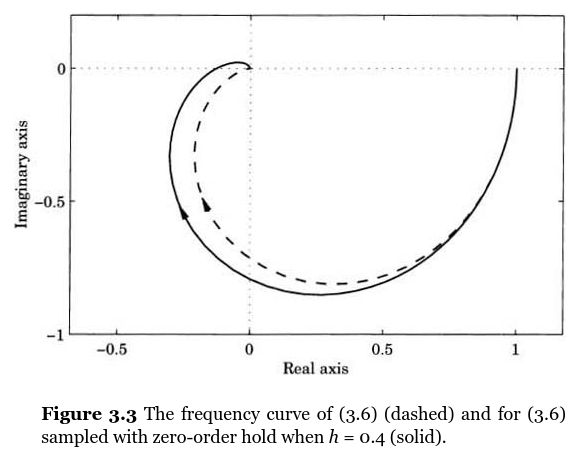
\includegraphics[width=0.5\linewidth]{../../figures/fig3-3.png}
\tiny Source: Åström \& Wittenmark
\end{center}
\end{frame}

\begin{frame}[label={sec:org2940ec7}]{The effect of sampling on the stability margins}
\[G(s) = \frac{1}{s^2 + 1.4s + 1} \quad \overset{h=0.4}{\longrightarrow} \quad H(z) = \frac{0.066z + 0.055}{z^2 - 1.450z + 0.571}\] 

\begin{center}
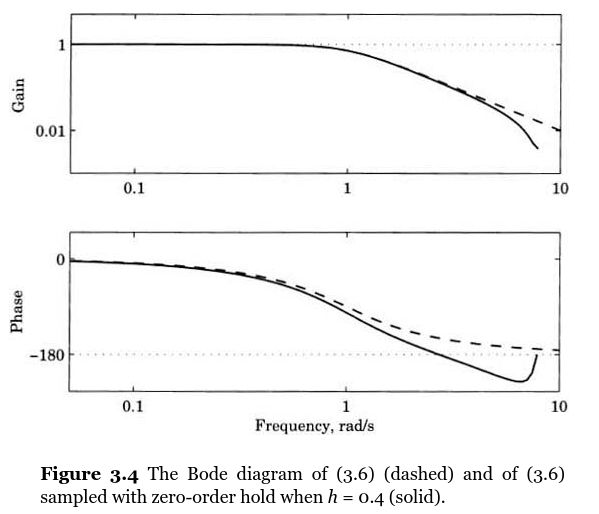
\includegraphics[width=0.5\linewidth]{../../figures/fig3-4.png}
\tiny Source: Åström \& Wittenmark
\end{center}
\end{frame}

\begin{frame}[label={sec:org666f404}]{Selecting the sampling period}
One can use the phase margin to determine a suitable sampling period. Given a desired cross-over frequency \(\omega_c\) and a maximum acceptable negative change in the phase margin  \(\Delta\varphi \approx 5^\circ\; - \; 15^\circ \approx 0.09 \text{rad}\; - \; 0.26\text{rad}\) (a rule-of-thumb).

\begin{center}
  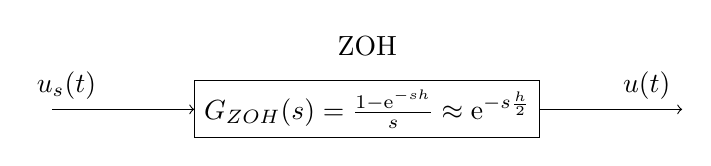
\begin{tikzpicture}[node distance=22mm, block/.style={rectangle, draw, minimum width=15mm}, sumnode/.style={circle, draw, inner sep=2pt}]

    \node[coordinate] (input) {};
    \node[block, right of=input, node distance=40mm] (plant)  {$G_{ZOH}(s) = \frac{1 - \mathrm{e}^{-sh}}{s}\approx \mathrm{e}^{-s\frac{h}{2}}$};
    \node[coordinate, right of=plant, node distance=40mm] (output) {};

    \draw[->] (input) -- node[above, pos=0.1, ] {$u_s(t)$} (plant);
    \draw[->] (plant) -- node[above, near end,] {$u(t)$} (output);
    \node[above of=plant,  node distance=8mm] {ZOH};
  \end{tikzpicture}
\end{center}
\[ \arg G_{ZOH}(i\omega_c) \approx \arg \mathrm{e}^{-i\omega_c \frac{h}{2}} = -\omega_c \frac{h}{2} \approx -0.09 \text{rad}\; - \; -0.26\text{rad} \]

\alert{Activity} Use the rule-of-thumb above to calculate a sampling period for the case  \(\omega_c = \unit{20}{\rad\per\second}\) and \(\Delta\varphi = \unit{0.2}{\rad}\).
\end{frame}
\end{document}